\section{Euclidean Voronoi Diagrams}
In this section we focus on the Voronoi diagram when the norm is the Euclidean norm, that is $\norm{\,\cdot\,}_2$. Here is the example from earlier:
\begin{figure}[H]
    \centering
    \subfloat{
      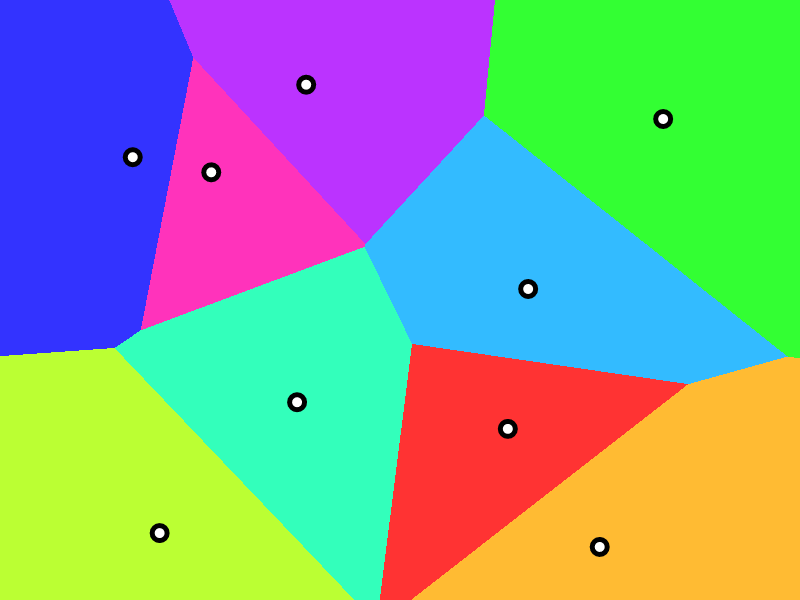
\includegraphics[scale=0.21]{naive-voronoi-L2}
    }
    \subfloat{
      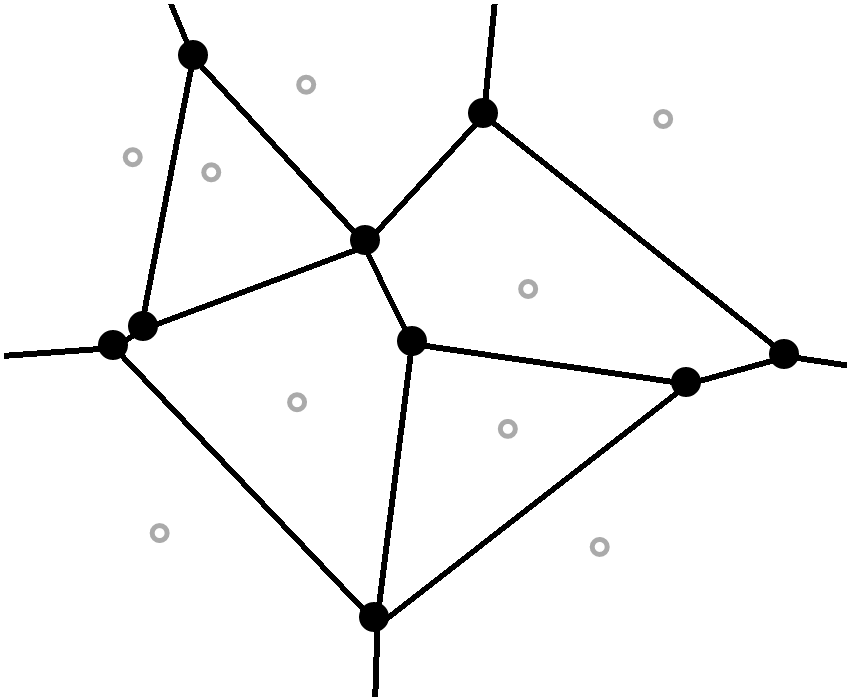
\includegraphics[scale=0.18]{naive-voronoi-graph-L2}
    }
\end{figure}
From linear algebra we know that $\norm{v}_2 = \sqrt{\ip{v}{v}}$, where $\ip{\,\cdot\,}{\,\cdot\,}$ is the usual dot product on $\R^2$. Given two points $p, q \in \R^2$ then the \textbf{bisector} of $p$ and $q$ is denoted by $\bi(p, q) \subset \R^2$ and denotes the set of points on a line $\ell$ which passes through the midpoint of $p$ and $q$ and is orthogonal (w.r.t. $\ip{\,\cdot\,}{\,\cdot\,}$) to the vector $p - q$.
\[
    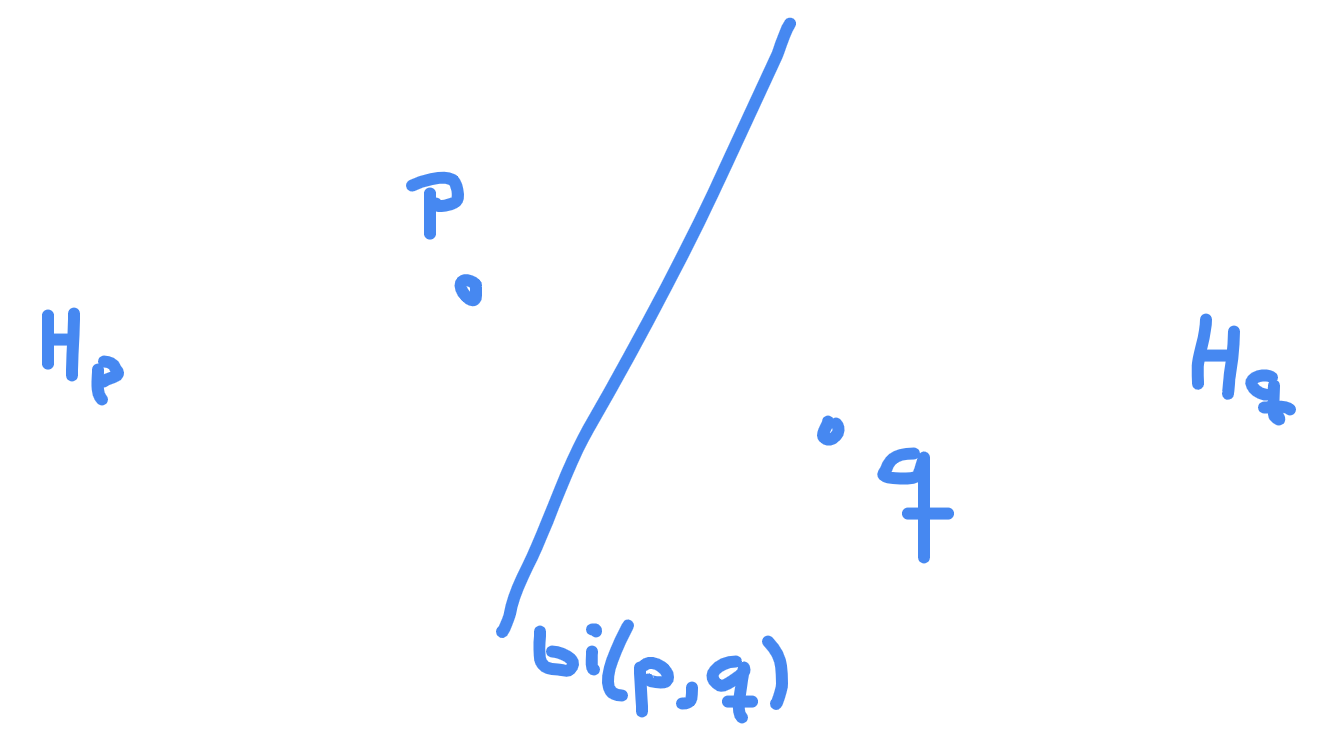
\includegraphics[scale=0.22]{temp-fig-2}
\]
A bisector $\bi(p, q)$ splits the plane into two \textbf{half-planes} $H_p$ and $H_q$ such that $p \in H_p$ and $q \in H_q$. We define $h(p, q)$ to be the open half-plane which contains $p$, that is the interior of $H_p$. So we have that
\[
    \R^2 = h(p, q) \cup \bi(p, q) \cup h(q, p).
\]
\begin{prop} \label{prop:hyperplaneinclusionproperty}
$r \in h(p, q)$ if and only if $\dist(r, p) < \dist(r, q)$.
\end{prop}
\begin{proof}
\[
    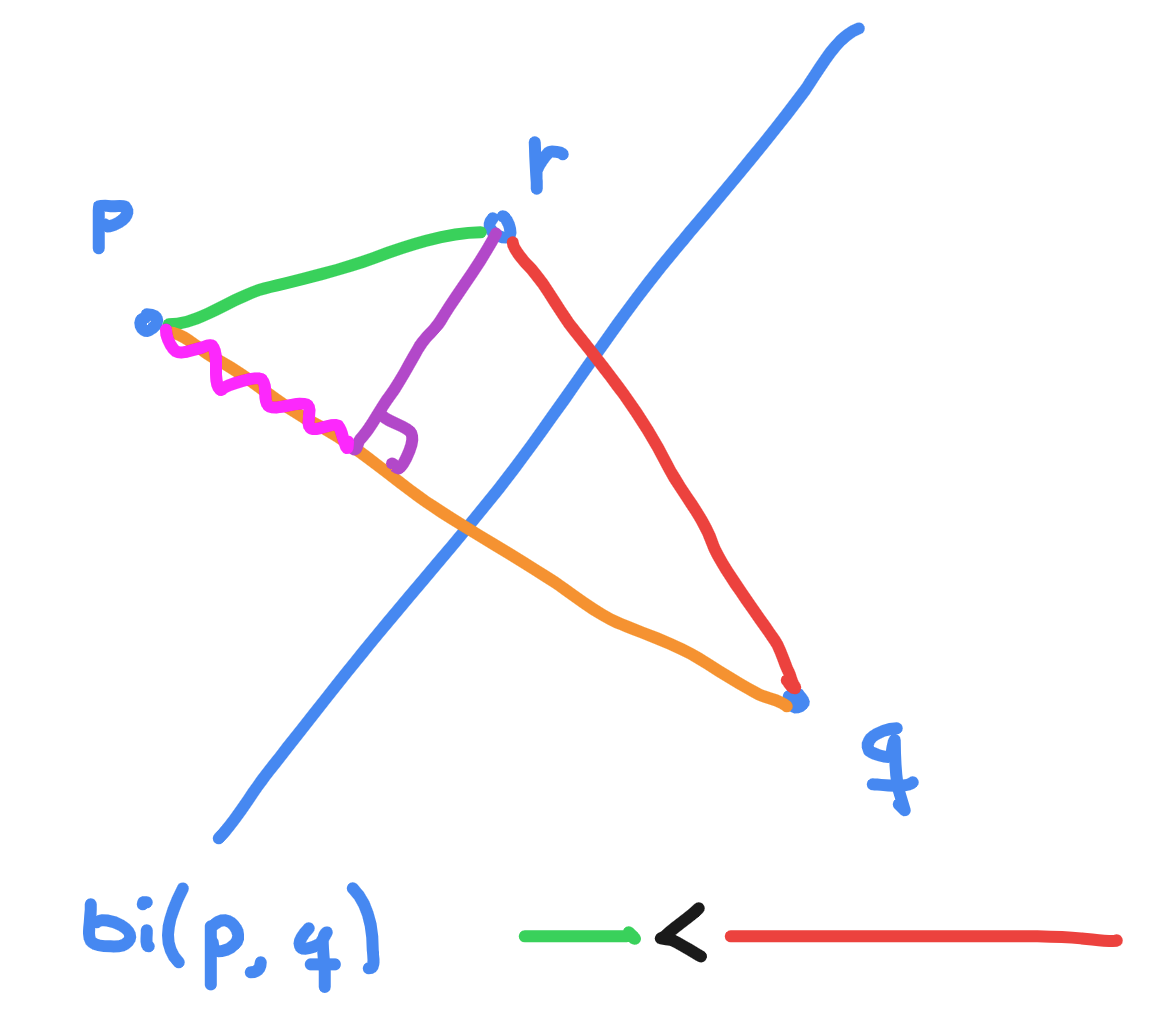
\includegraphics[scale=0.25]{temp-fig-1}
\]
\todo{Formalize} Proof sketch: We want to project $r$ onto the orange line. As long as $r \in H_p$ then the squiggly pink segment is shorter than the orange segment, which will make the green segment shorter than the red segment (which is what we want to show).
\end{proof}

\begin{prop} \label{prop:cellsareintersectionsofhalfplanes}
For every Voronoi cell we have
\[
    \mathcal{V}(p_i) = \bigcap_{\substack{1 \leq j \leq n \\ j \ne i}} h(p_i, p_j).
\]
\end{prop}
\begin{proof}
``$\subset$'': Let $r \in \mathcal{V}(p_i)$. Then $\dist(r, p_i) < \dist(r, p_j)$ for all $i \ne j$. Prop \ref{prop:hyperplaneinclusionproperty} then gives us that this is equivalent to $r \in h(p_i, p_j)$ for all $i \ne j$.

``$\supset$'': This argument is symmetrical to the above argument.
\end{proof}
A Voronoi cell is thus the intersection of convex sets and is therefore convex. We conclude that the Voronoi cells are open and convex (possibly unbounded) polygons with at most $n - 1$ vertices and $n - 1$ edges. \\

We now look at the shape of the entire Voronoi diagram:
\begin{thm}
If the points in $P$ are collinear then $\Vor(P)$ consists of $n - 1$ parallel lines. Otherwise, $\Vor(P)$ is connected and its edges are either segments or half-lines.
\end{thm}
\begin{proof}
\todo{.}
\end{proof}

Finally, we show that that the complexity of the vertices and edges is $\mathcal{O}(n)$:
\begin{thm}
For $n \geq 3$, the number of vertices in $\Vor(P)$ at most $2n - 5$ and the number of edges is at most $3n - 6$.
\end{thm}
\begin{proof}
\todo{.}
\end{proof}